\section{Jegyzet összefoglaló}

\subsection{Alapfogalmak}

	\textit{Adatbázis kezelő}t jellemző tulajdonságok:
	\begin{itemize}
		\item nagy adatmennyiség
		\item gazdak struktúra
		\item hosszú életciklus
	\end{itemize}

	\textbf{HDD} vel foglalkozunk ( mágneslemezes tár)

\subsection{Relációk}

	\textbf{Reláció számossága:} A sorok száma

	\textbf{Reláció aritása:} Attribútumok/Oszlopok száma

\subsection{Relációs lekérdezések optimalizálása}


	\begin{center}
		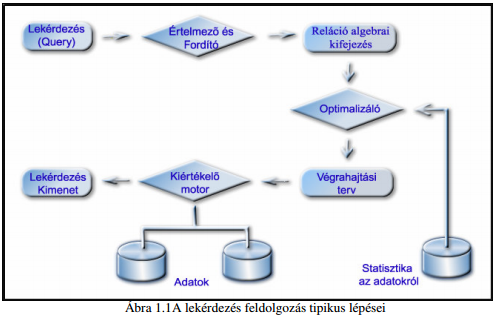
\includegraphics[scale=0.8]{img/opt1}
	\end{center}

Lépések:
	\begin{enumerate}
		\item \textbf{Fordítás}

			PL: SQL nyelvét szintaktikailag ellenőrizzük és ha helyes egy Reláció algebrai kifejezésre képezzük le

		\item \textbf{Végrehajtási terv készítése az adatok alapján}

			Egy adott lekérdezést többféleképpen is el tudunk készíteni, ezek közül a legoptimálisabbat keressük.\\[-2pt]

		A \textit{katalógusban} adatokat találunk a relációkról:

				\begin{itemize}
					\item $n_r$(number) : az r relációban lévő rekodok száma

					\item $b_r$(blocks) : az r relációban lévő rekordokat tartalmazó blokkok száma

					\item $s_r$(size) : egy rekord nagysága byte-okban

					\item $f_r$(blocking factor): mennyi rekord fér el egy blokkba

					\item $V(A,r)$(Values): Hány különböző értéke fordul elő az A atribútumnak az r relációban

						 \forceindent V(A,r) = $| \pi_A(r)|$; Ha A kulcs $\rightarrow$ V(A,r) = $n_r$ ( sorok száma )

					\item SC(A,r) (Selection Cardinality): Azon rekordok átlagos száma, amelyek kielégítenek egy egyenlőségi feltételt az A attribútumra feltéve, hogy legalább egy rekord kielégíti ezt az egyenlőségi feltételt.

					\forceindent SC(A,r) = $\dfrac{n_r}{V(A,r)}$, Ez csak akkor igaz ha egyenletesen oszlanak el a különböző értékek

					\forceindent Ha A kulcs $\rightarrow$ SC(A,r) = 1

				\end{itemize}
			Egyéb adatok B* fák/Hash tábákról

				\begin{itemize}
					\item $f_i$ : Az átlagos pointer-szám a fa struktúrájú indexek csomópontjaiban, mint pl. a B* fáknál, azaz a csomópontokból induló ágak átlagos száma

					\item $HT_i$ (Height of tree) : Az i index szinjeinek a száma, azaz az index magassága B* fáknál

						\forceindent B* $\rightarrow HT_i = | log_{f_i} V(A,r) |$ Hash-indexnél $\rightarrow HT_i = 1$

					\item $LB_i$(Lowest level index Block): Az i index legalsó szintű blokkjainak a száma, azaz a levélszintű indexblokkok száma
				\end{itemize}

			\textbf{Keresési (szelekciós) algoritmusok:}
			\begin{enumerate}
				\item Alap algoritmusok:
					\begin{enumerate}
						\item Lineáris keresés: $E = b_r$

						\item Bináris keresés: $E = \lceil log_2 b_r \rceil + \left\lceil \dfrac{SC(A,r)}{f_r} \right\rceil -1$

							\forceindent Megtalálás $log_2$ utána még van $SC / f_r$ rekord, -1 pedig azért mert az első blokk az bennevan a megtalálásba
					\end{enumerate}

				\item Indexelt szelekciós algoritmusok
				\begin{itemize}
					\item Elsődleges index:

						\forceindent Az elsődleges index a rekordok olyan sorrendben való olvasását teszi lehetővé, amely megfelel a rekordok fizikai tárolási sorrendjének. Egyébként Másodlagos Index.

					\item Másodlagos index:\\[1pt]
				\end{itemize}


					\begin{enumerate}
						\item Elsődleges indexel, egyenlőségi feltételt a kulcson vizsgálva.

							\forceindent  $E = HT_i + 1$

						\item Elsődleges index, de egyenlőségi feltétel nem a kulcson

							\forceindent $E = HT_i + \left\lceil \dfrac{SC(A,R)}{f_r} \right\rceil $

						\item Másodlagos index használatával

							\forceindent $E = HT_i + SC(A,r)$

							\forceindent $E = HT_i + 1$ ha A egyediséget biztosít

					\end{enumerate}

				\item Összehasonlítás alapú szelekció

					\begin{enumerate}
						\item Elsődleges indexel: $E = HT_i + br/2$

						\item Másodlagos index: $ E = HT_i + \dfrac{LB_i}{2} + \dfrac{n_r}{2}$
					\end{enumerate}

			\end{enumerate}


				\textbf{Join típusok}
					\begin{center}
						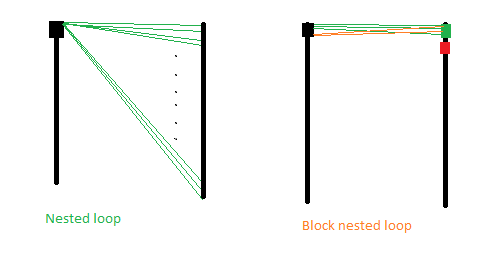
\includegraphics[scale=0.7]{img/JoinTypes}
					\end{center}

					\begin{enumerate}
						\item Nested-loop join:  $b_r + n_r \cdot b_s$\quad -  2 for ciklus

								\forceindent minden $n_r$ rekordhoz beolvasom a hozzá tartozó $b_s$ blokkot és még beolvasom az összes $b_r$ blokkot is.

						\item Block nested -loop join : $b_r \cdot b_s + b_r$

							\forceindent Kihasználja hogy blokkok kerülnek a memóriába, 1-1 beolvasott blokk összes összehasonlítása, majd újabb blokk beolvasása. A képen a piros blokk csak akkor kerül beolvasásra ha fekete-zöld blokk összes rekordja össze volt már hasonlítva.

						\item Indexed nested-loop join: $b_r + n_r \cdot c$ \quad ahol \textit{c} a szelekció költsége s-en

						\item Merge join: $b_r + b_s + a$ \quad - ahol a a rendezés költsége

						\forceindent Nagy adathalmazoknál általába ez a legoptimálisabb

						\item Hash join: $b_r + n_r \cdot h_s$ \quad - Ahol $h_s$ egy blokk elérési ideje vödrön belül
					\end{enumerate}

				Kiértékelési terv készítésénél exponenciálisan növekszik a lehetséges elrendezések száma, a joinok számának növekedésével. Ezért egy lokálisan optimális megoldást választunk ki!


						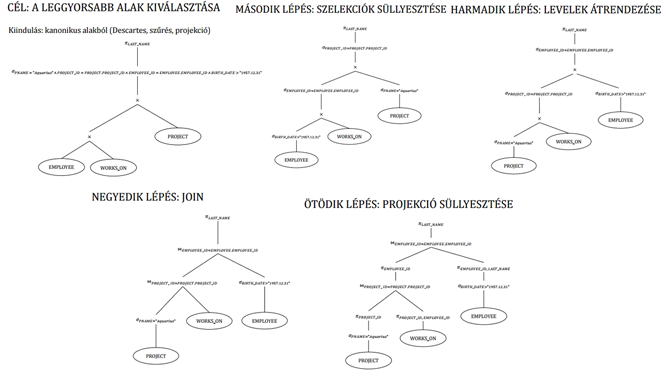
\includegraphics[scale=0.75]{img/optimalizalas}

	\end{enumerate}

\subsection{Hálós adatbázisok}

	Set típusok szintjén modellezünk\\[0pt]

  \begin{definicio}{Set típus}

		Legyen $R_1$ és $R_2$ két rekord típus és legyenek $F(R_1)$ és $F(R_2)$ a konkrét esetek halmazai. Ekkor az S set típust az $S := R_1 \times R_2$ művelettel definiálhatjuk, ami egy $F(R_2) \rightarrow F(R_1)$ függvényszerű kapcsolatot ír le. $R_1$ - \textit{owner} típus, $R_2$ - \textit{member} típus\\[1pt]

  \end{definicio}

	\textbf{Set}
		\begin{itemize}
			\item Egyenrangú \textit{member}-rekordoknak egy (akár üres) halmazából, és
			\item Pontosan egy \textit{owner}-rekodból áll, aminek a member-rekordok alárendeltek.
		\end{itemize}

\subsection{Objektumorientált adatbázis-kezelő rendszerek}

\textbf{Problémák a Relációs-adatbázisokkal:}

	\begin{enumerate}
		\item Nincsenek \textit{rekurzív} lekérdezések.

				PL: Dolgozók, beosztottak reláció

		\item "lista" jellegű információk tárolására nem alkalmas

			PL: Grafika: Egy fonal tetszőleges számú töréspontjának tárolása

		\item Autó,Garázs példa $\ldots$

	\end{enumerate}

\textbf{Típuskonstruktorok}

	\begin{itemize}
		\item Halmazkonstruktor: $T_{set} = \mathbf{SET}\ OF(A: T)$, ahol A attribútum, T pedig az attribútum típusa. A halmaz típus legfontosabb jellemzője, hogy elemei rendezetlenek.

		\item Listakonstruktor: $T_{list} = \mathbf{LIST}\ OF(A: T)$, ahol A attribútum, T pedig az attribútum típusa. A lista típusra jellemző, hogy elemei szekvenciálisan rendezettek. A progamozási nyelvek láncolt listájával analóg struktúra kialakítására ad lehetőséget.

		\item Tuplekonstruktor: $T{tuple} = \mathbf{TUPLE}\ OF(A_1 : T_1 , \ldots , A_n : T_n)$, ahol $A_i$ attribútum, $T_i$ pedig az $A_i$ attribútum típusa. A tuple típus a relációs modellben a reláció egy elemének felel meg. ( C struct)

	\end{itemize}

	Objektumok között asszociációk vannak. Ez lehet akár kétirányú is.

	PL:
	\begin{center}
		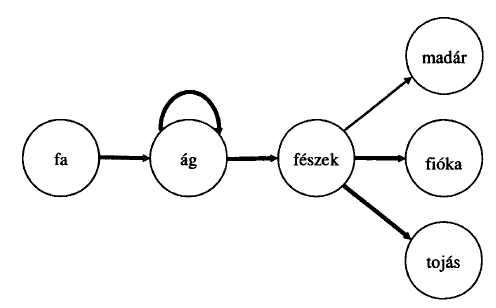
\includegraphics[scale=0.6]{img/fa}
	\end{center}

	Az ábrán vastaggal jelölt vonalak mentén terjed a terjedési tulajdonság. Ha valamelyik őse elpusztul akkor az összes vastaggal jelölt leszármazottja is ( rekurzió ). Ha elpuszul a fészek $\rightarrow$ elpusztulnak a fiókák, és a tojások, de a madarak nem.
